\documentclass[11pt]{article}

\usepackage{geometry}
\geometry{a4paper,left=31.7mm,right=31.7mm,top=25.4mm,bottom=25.4mm}
\usepackage{graphicx}
\usepackage{caption}
\usepackage{subfigure}
\usepackage{cite}
\usepackage{hyperref}

\hypersetup{hidelinks} 
\usepackage{amssymb}
\usepackage[inkscapelatex=false]{svg}
\usepackage{amsmath}
\numberwithin{figure}{section}
\numberwithin{equation}{section}
\newcommand\keywords[1]{\textbf{Keywords}: #1}

\title{\vspace{20 pt}\huge{OFDM Modulation for 4G LTE Mobile}\\\vspace{10 pt}\large{EEEE3087 Mobile technologies|Coursework1}\vspace{100 pt}}
\author{\huge{Yaowen Hu}\\{\small 20495331}}
\date{}

\hypersetup{
pdftitle={OFDM Modulation for 4G LTE Mobile},
pdfauthor={Yaowen Hu},
pdfsubject={EEEE3087 Mobile technologies|Coursework1},
pdfkeywords={OFDM, QAM, BER}
}

\begin{document}
%%%%%%%%%%%%%%%%%%%%%%%%%%%%%%%%%%%%%%%%%%%%%%%
\begin{titlepage}
\begin{figure}
    \vspace{30 pt}
    \centering
    
\includegraphics[width=0.9\textwidth]{images/logo.png}
\end{figure}

\vfill
\maketitle
\vspace{120 pt}
\centering{Module Convenor:}\\
\centering{Dr Steve Greedy}\\
\centering{Dr Minglei You}\\
\centering{Dr Paul Blunt}\\
\vfill

\centering{University of Nottingham}\\
\vspace{10 pt}
\centering{\today}
\thispagestyle{empty}
\pagebreak
\end{titlepage}

%%%%%%%%%%%%%%%%%%%%%%%%%%%%%%%%%%%%%%%%%%%%%%%
\begin{abstract}
% \addcontentsline{toc}{section}{Abstract}
OFDM technology started to become rapidly popular after the 1990s. This paper introduces the main principles and implementation of OFDM, and introduces the important role of OFDM at the level of 4G and 5G mobile networks. In the second part, I have done the simulation of a 16-QAM based OFDM transceiver in Simulink$^\circledR$ and observed the constellation diagram, power spectrum and calculated the BER.

Through this article, I learned how OFDM is implemented and how to complete a complete transceiver design in Simulink$^\circledR$ and understand the impact of different channels and different signal-to-noise ratios on communication quality.
\end{abstract}
\keywords{OFDM, QAM, BER}
\pagenumbering{Roman}
\setcounter{page}{1}
\thispagestyle{plain}
\pagebreak
%%%%%%%%%%%%%%%%%%%%%%%%%%%%%%%%%%%%%%%%%%%%%%%
\tableofcontents
\thispagestyle{empty}
\pagebreak
%%%%%%%%%%%%%%%%%%%%%%%%%%%%%%%%%%%%%%%%%%%%%%%
\part{Introduction and Background Research}

\pagenumbering{arabic}
\pagestyle{plain}
\setcounter{page}{1}

\section{Introduction}
\textit{Orthogonal Frequency Division Multiplexing} (OFDM) is one of the most powerful modulation techniques. It is designed for high-data-rate transmission. In general, it will convert a high-rate data stream into several low-rate data streams which can be transmitted in parallel\cite{RN79}. These streams or sub-carriers are orthogonal to each other, which means they don't interfere with each other, allowing multiple sub-carriers to be transmitted simultaneously over the same channel without causing interference. Figure \ref{fig:subcarriers} shows the spectrum of sub-carriers of OFDM, as you can see all the sub-carriers do not overlap and they are orthogonal to each other \cite{RN80}.
\begin{figure}[!ht]
    \centering
    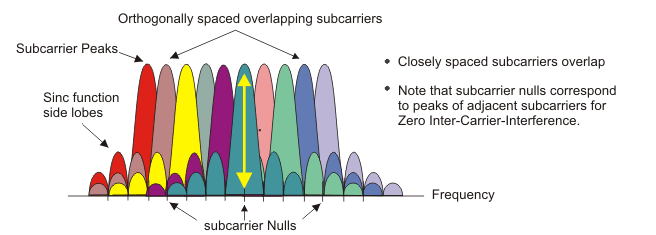
\includegraphics[width=1\textwidth]{images/subcarriers1.png}
    \caption{\label{fig:subcarriers}The spectrum of sub-carriers of OFDM}
\end{figure}
\subsection{A Brief Implementation of OFDM}
At the transmitter, it is required to apply a series-parallel (SP) conversion, i.e., from a single point to N points. Then use \textit{Inverse Fast Fourier Transform} (IFFT) to create the time-domain OFDM signal from the modulated signal. In the end, add a \textit{Digital-to-Analogue Converter} (DAC) to from the signal which can be transmitted in the channel.

At the receiver, the OFDM signal is first demodulated to recover the sub-carriers. Then, each sub-carrier is processed individually to recover the raw data. A parallel-serial converter is then used to convert the low-speed data stream to a high-speed data stream for use by the terminal.

Overall, the principle of OFDM allows for high-speed data transmission over limited bandwidth channels, with robustness against interference and distortion caused by multi-path propagation. 
\subsection{Role in Mobile Networks}
OFDM plays an important role in both 4G and 5G LTE (Long-term Evolution) mobile networks.
\begin{itemize}
    \item Strong anti-interference capability:When the signal is transmitted in the air, it is very likely to be interfered and distorted by multi-path propagation which is shown in Figure \ref{fig:multipath propagation}. Hence, people are considering transmitting multiple non-interference sub-carriers which can be recovered easily by their orthogonality.
    \begin{figure}[!ht]
        \centering
        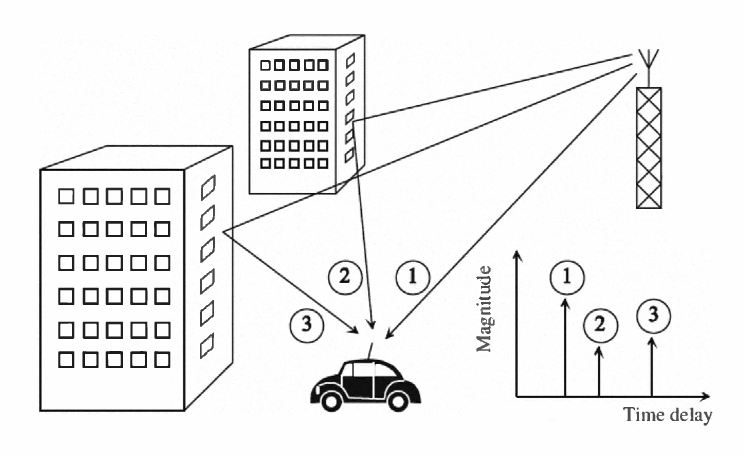
\includegraphics[width=0.7\textwidth]{images/multipath propagation.png}
        \caption{\label{fig:multipath propagation}The multi-path propagation}
    \end{figure}
    \item High data rates: As OFDM owns several channels to transmit data, it can gain higher rates. That is, it can be considered as a \textit{Multiple-Input Multiple-Output} (MIMO) system.
    \item High spectrum utilization: OFDM can be used to transmit multiple sub-carriers simultaneously over the same channel, which can be used to increase the spectral efficiency of the system.
\end{itemize}

OFDM is used in many different communication systems, including digital television, Wi-Fi, 4G and 5G LTE  mobile networks, and \textit{Digital Subscriber Line} (DSL) modems over copper-based telephone access lines. Due to its excellent performance, OFDM has been standardized by IEEE into standards such as 802.11g and 802.11a. The \textit{asynchronous digital subscriber line} (ADSL) and \textit{high-bit-rate digital subscriber line} (HDSL) technologies use OFDM for fixed-wire applications.\cite{RN78, RN79}.

\section{Implementations of OFDM Based on QAM}
\subsection{QAM Modulation}
\textit{Quadrature Amplitude Modulation} (QAM) is a digital modulation which uses two sinusoidal carriers that have a phase difference of $\pi/2$, known as orthogonality or quadrature. Each of them can be modulated independently, transmitted over the same frequency band, and demodulated at the receiver. Both mobile radio and satellite communication technologies use QAM and its variations \cite{RN77}.

Based on this theory, there are many QAM variants, such as 64-QAM, 256-QAM, 1024-QAM, which are widely used \cite{RN77}. The diagram below shows the constellation of QAM.
\begin{figure}[!h]
    \centering
    \includesvg[width=0.45\textwidth]{images/constellation_for_QAM.svg}
    \caption{Constellation plot for 4-QAM, 16-QAM, 32-QAM, and 64-QAM}
    \label{fig:Constellation of QAM}
\end{figure}
\subsection{Implementations of Transceiver}
\subsubsection{Implementations of QAM}
When the signal is sent under the QAM modulation, it will change the amplitude and phase of it. 

One possible and easiest way to implement is generate two carrier which are sine and cosine. They are obviously quadrature. The symbols that go through the cosine carrier are called \textit{in-phase} (I) signal and the others are called \textit{quadrature} (Q). They can be represented as: 
\begin{equation}
I = A\cos{\varphi} \label{con:i signal}
\end{equation}
and
\begin{equation}
Q = A\sin{\varphi} \label{con:q signal}
\end{equation}
After that, mix these two signals. This modulation scheme is called 4QAM, and in fact, it is not different from \textit{Quadrature Phase Shift Keying} (QPSK).

At the same time, we can increase the order of QAM. M-decimal QAM is denoted as MQAM. As an example, I will briefly describe 16-QAM. The 16-QAM modulation scheme is shown in Figure \ref{fig:structure of QAM}.
\begin{figure}[!ht]
    \centering
    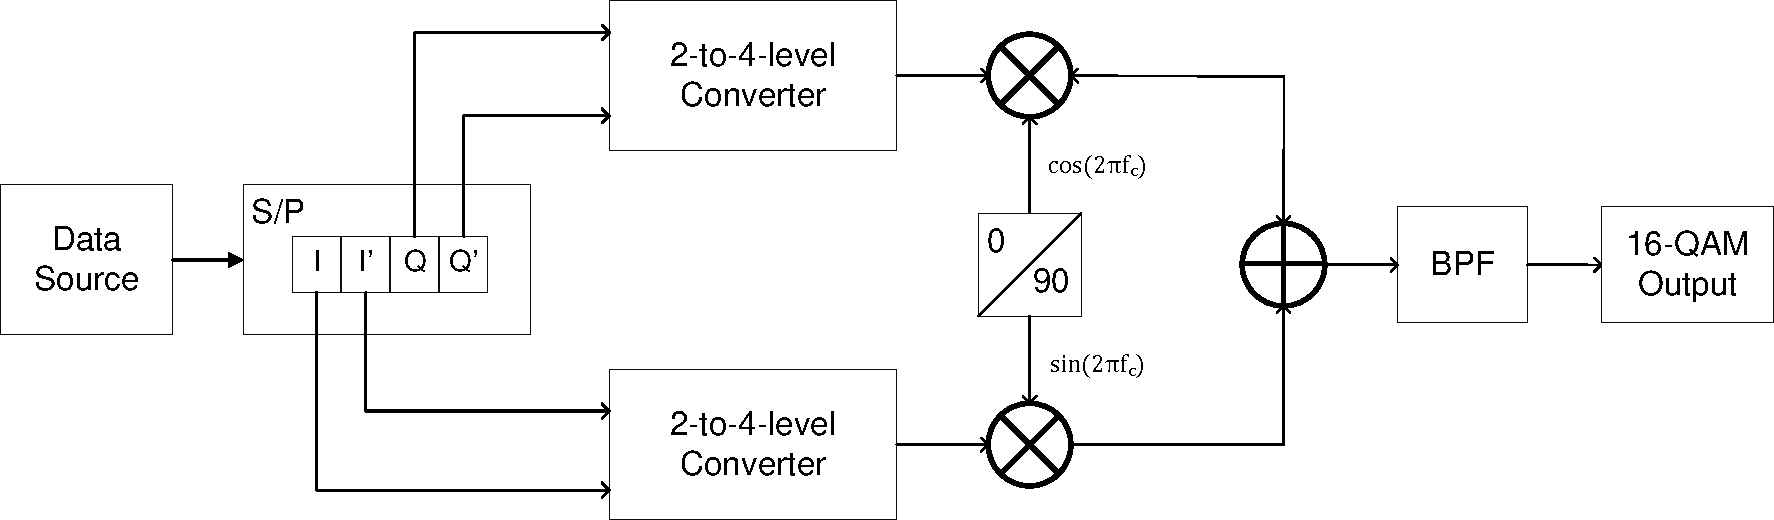
\includegraphics[width=0.8\textwidth]{images/16QAM.pdf}
    \caption{Block diagram of 16-QAM modulator}
    \label{fig:structure of QAM}
\end{figure}

Mathematically, it can be expressed as,
\begin{equation}
S_{16-QAM}(t) = I(t)\cos{2\pi f_ct}-Q(t)\sin{2\pi f_ct} \label{con:16-QAM}
\end{equation}
where $I(t)=\pm 1,\pm 3$; $Q(t)=\pm 1,\pm 3$. Since there are 16 possible combinations of $I(t)$ and $Q(t)$, the synthesized QAM signal has 16 states. In a period, there will be $log_216=4$ bits to be transmitted, and it will increase the data rate. Hence, we will use the \textit{Series-Parallel} (SP) conversion, i.e., from a single point to N points. In this scenario, $N=2$. In the I/Q channel respectively apply a 2-to-4 level converter. This mapper will transfer the four combinations of two bits into four amplitude levels. After that, the I/Q channel will multiply by the sine and cosine waves. 
\subsubsection{Implementations of OFDM}
In order to make their sub-carriers orthogonal to each other or not overlap each other in the frequency domain, the inner product of any two sub-carriers is zero. That is, in the time domain, the cross-correlation of any two sub-carriers is zero. As shown in the following Equation \ref{con:cc},
\begin{equation}
(f \star g) \triangleq \int_{-\infty}^{\infty} sub-carrier_N(t) \cdot sub-carrier_{N+1}(t)dt=0 \label{con:cc}
\end{equation}
Before mapping each low-rate date to sub-carriers, we first need to use a serial to parallel converter. The IFFT can be performed only after SP conversion. At the same time, this operation corresponds to an N-fold increase in the duration of each symbol, increasing the system's immunity to interference.

Secondly, it's common to use the \textit{Inverse Discrete Fourier Transform} (IDFT) technique to map to sub-carriers. The IDFT can be represented as: 
\begin{equation}
\hat{x}[k]=\sum_{n=0}^{N-1} e^{-i\frac{2\pi}{N}nk}x[n] \qquad k = 0,1,\ldots,N-1. \label{con:idft}
\end{equation}
We usually us the \textit{Inverse Fast Fourier transform} (IFFT) technique to complete that as it will perform a more efficient way to compute. The process of generating an OFDM signal using IFFT involves taking the data to be transmitted and mapping it onto the sub-carriers. The sub-carrier signals are then modulated using the appropriate phase and amplitude information, and then combined using the IFFT to create the time-domain OFDM signal. 

At the receiver, the process is reversed. When the signal passes through the channel, it is first sampled. Then, a PS converter is used to feed the FFT with sub-carriers. After that, write a block of N symbols into a vector which is PS converter. Hence, the structure of OFDM transceiver is shown in the Figure \ref{fig:Transceiver structure}.
\begin{figure}[!ht]
    \centering
    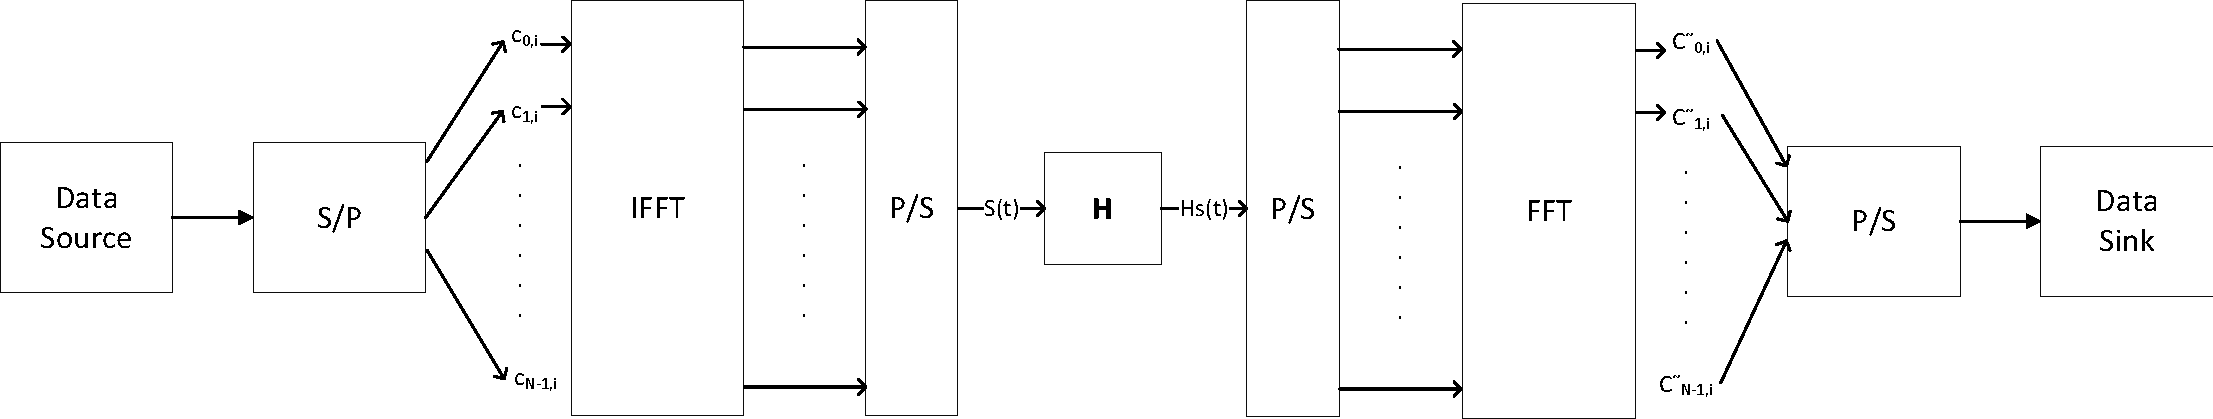
\includegraphics[width=0.9\textwidth]{images/OFDM_transceiver.pdf}
    \caption{Structure of OFDM Transceiver}
    \label{fig:Transceiver structure}
\end{figure}
\subsubsection{Typical BER}
In order to provide a typical \textit{Bit Error Rate} (BER) of OFDM and 16-QAM, I use MATLAb to simulate the BER of OFDM and 16-QAM. The simulation results are shown in the Figure \ref{fig:BER of OFDM and 16-QAM}.
\begin{figure}[!h]
    \centering
    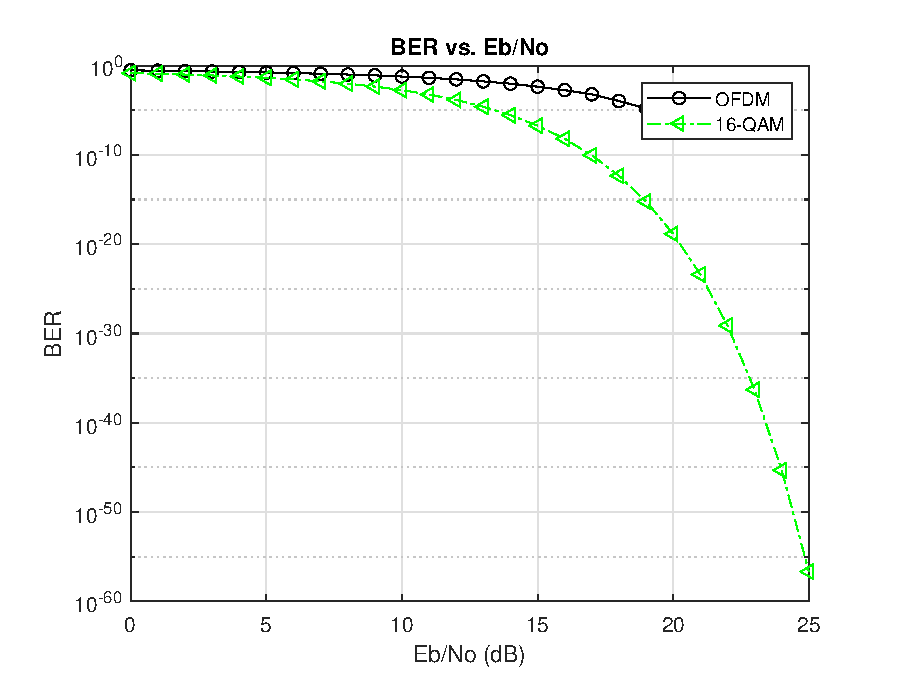
\includegraphics[width=0.8\textwidth]{images/typical_BER.eps}
    \caption{Typical BER of OFDM and 16-QAM}
    \label{fig:BER of OFDM and 16-QAM}
\end{figure}
\subsection{Advantages and Disadvantages}
When OFDM was first invented in the 1960s at Nokia Bell Lab \cite{RN82}, it was not taken seriously because of several technical limitations that made it challenging to implement in practical communication systems. Some of these limitations include: high complexity, sensitivity to frequency offset, limited channel estimation and so on. It was not until the 1990s, when advances in DSP, computing technology and FFT algorithms, made it possible to overcome these technical limitations, that OFDM started to gain widespread attention and adoption in communication systems. 

Its advantages includes robustness in the presence of multi-path transmission, relative insensitivity to timing offsets, compatibility with MIMO systems and the ability to support multiple access in the form of \textit{Orthogonal Frequency Division Multiple Access} (OFDMA). 

Though, it still has some drawbacks, high \textit{Out-of-Band} (OOB) power, sensitivity to frequency offset, and high \textit{Peak-to-Average Power Ratio} (PAPR) \cite{RN81}.

\section{Practical OFDM Modulator or Demodulator Design}
The most ordinary way to implement OFDM digitally on hardware is using \textit{Field Programmable Gate Array} (FPGA). However, when the OFDM is invented, there are still many ways to implement it in an analogue circuit. The the structure of OFDM transceiver implementing in analogue circuit is shown in the Figure \ref{fig:Transceiver structure analogue} \cite{RN79}.
\begin{figure}[!h]
    \centering
    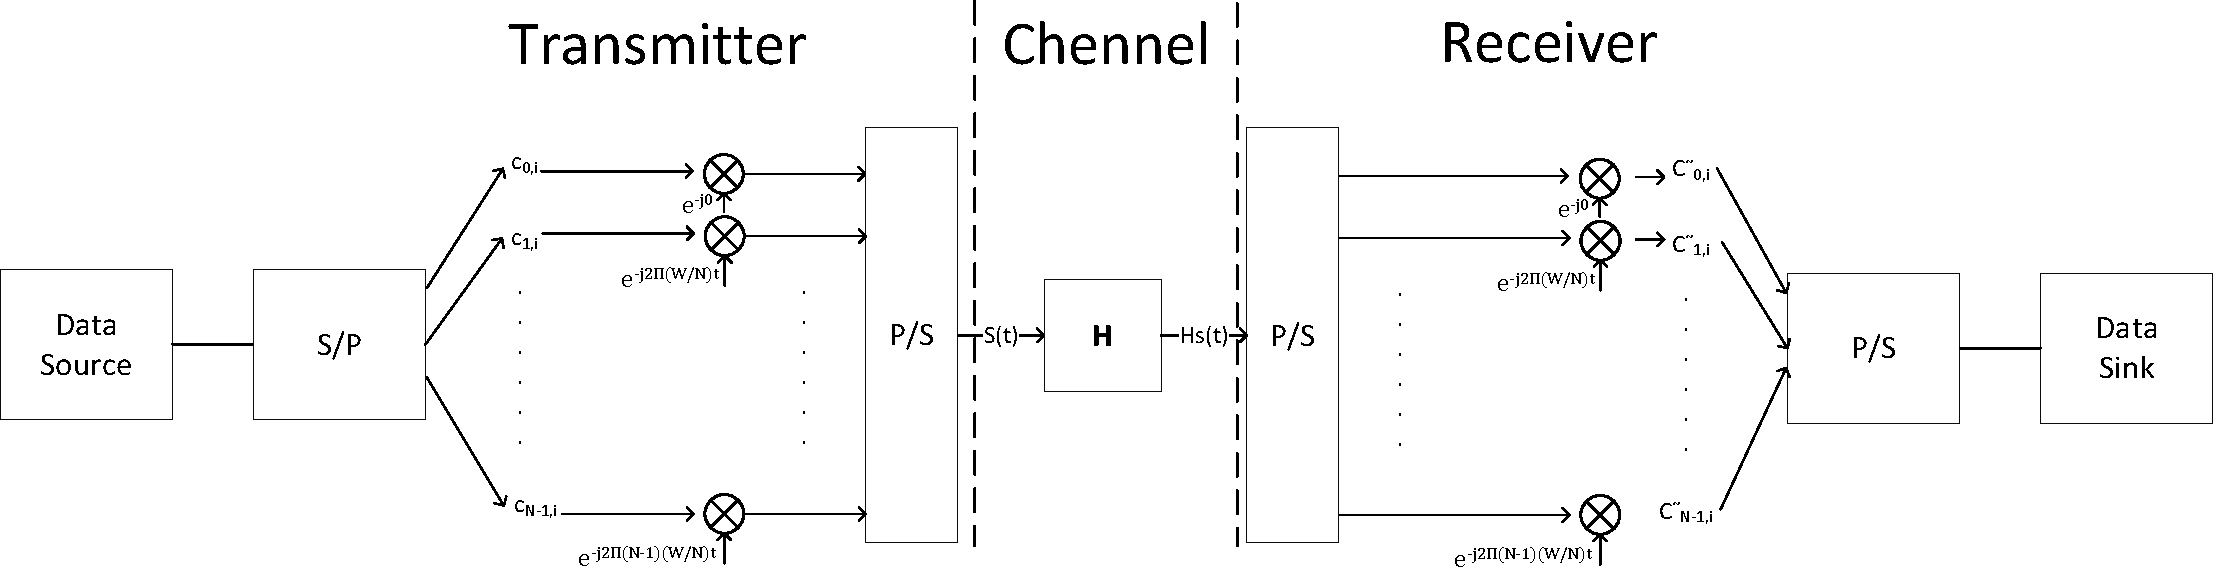
\includegraphics[width=0.9\textwidth]{images/OFDM_transceiver_analog.pdf}
    \caption{Structure of OFDM Analogue Transceiver}
    \label{fig:Transceiver structure analogue}
\end{figure}
We can use an oscillator to generate a continuous wave (CW) signal, and then use a frequency multiplier and a comb generator to generate the subcarriers at the desired frequencies. The comb generator can be implemented using a phase-locked loop (PLL) or a delay-line filter. The subcarriers are then modulated using QAM or other modulation schemes, and combined using a mixer and a filter to generate the final OFDM signal.
\begin{itemize}
    \item Mixer: Mixer is an important device in the RF circuit, it is often used for modulation, the signal will be loaded on the high frequency signal.
    \begin{figure}[!h]
        \centering
        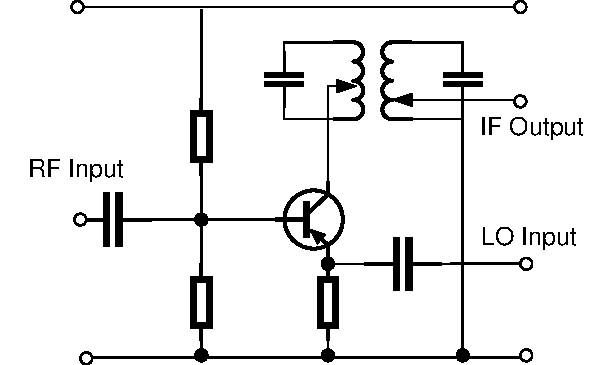
\includegraphics[width=0.5\textwidth]{images/mixer.pdf}
        \caption{Schematic of a Mixer}
        \label{fig:mixer}
    \end{figure}
    \item LPF: \textit{Low Pass Filter} (LPF) is a filter that passes low-frequency signals and attenuates high-frequency signals. It is very useful in the analogue OFDM transceiver.
    \begin{figure}[!h]
        \centering
        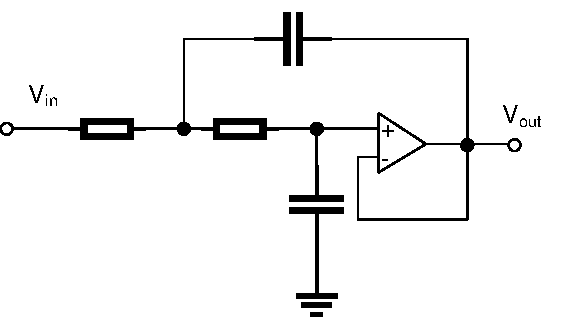
\includegraphics[width=0.5\textwidth]{images/LPF.pdf}
        \caption{Schematic of a LPF}
        \label{fig:LPF}
    \end{figure}
\end{itemize}
%%%%%%%%%%%%%%%%%%%%%%%%%%%%%%%%%%%%%%%%%%%%%%%
\part{BER Analysis}
\section{Blocks of the OFDM Transceiver in Simulink$^\circledR$}
\begin{figure}[!h]
    \centering
    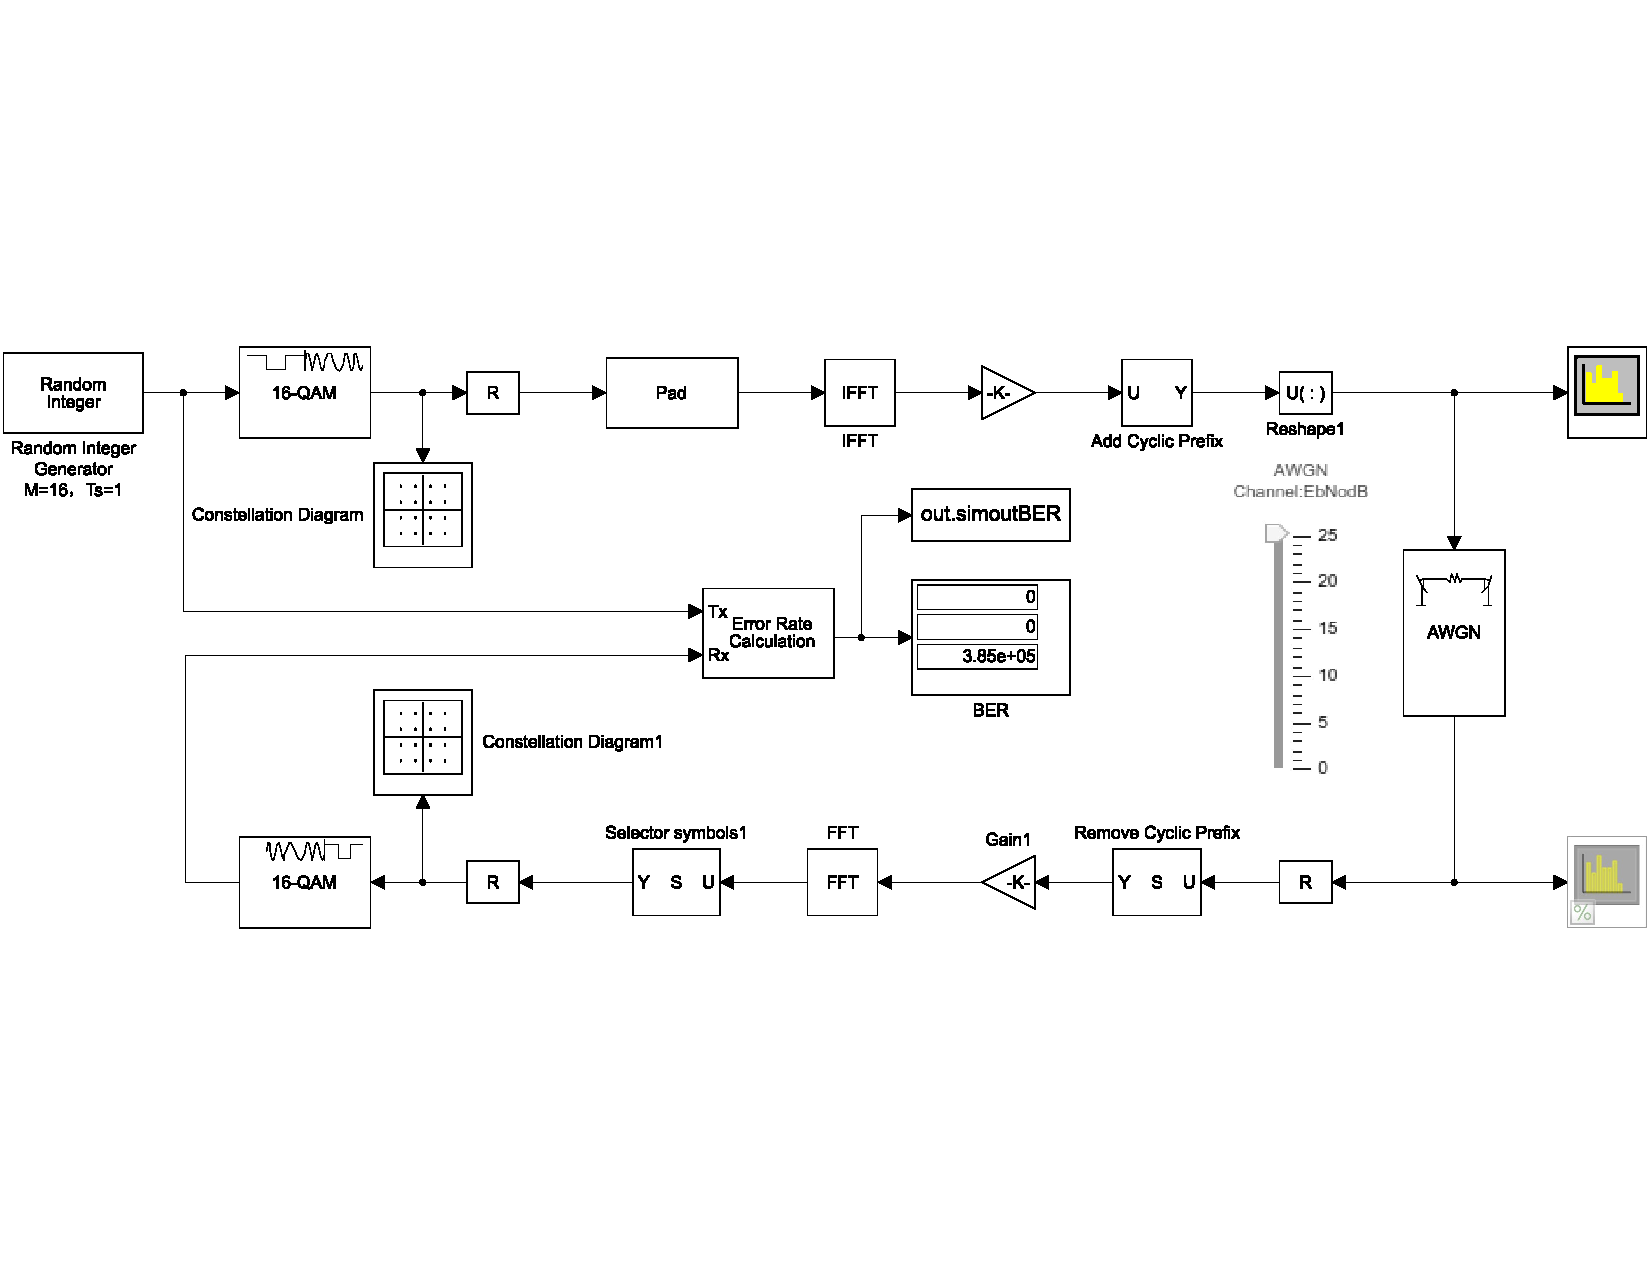
\includegraphics[width=0.9\textwidth]{images/simulink.pdf}
    \caption{Schematic of 16-QAM-based OFDM transceiver}
    \label{fig:simulink}
\end{figure}
A simulation software called Simulink$^\circledR$ is frequently used in the planning and evaluation of communication systems, including OFDM. Simulink$^\circledR$ offers a graphical interface for creating communication system models, making it simpler to develop and test various OFDM system configurations. Figure \ref{fig:simulink} shows the full schematic of 16-QAM-based OFDM transceiver.
\begin{itemize}
    \item Random Integer Generator: This block can provide a random sequence of numbers as the input raw data.
    \item 16-QAM: This block can modulate or demodulate the data by 16-QAM modulation. This process is called baseband modulation. After that, we can convert baseband signals into frequency band signals and map the data to I/Q.
    \item Reshape + Padding: This block can reshape the data into a matrix and add some zeros to the end of the data to make the length of the data can be divided by 64. They are designed to generate OFDM symbols.
    \item IFFT: This block can map the OFDM symbols into time domain signals. The subcarrier signals are then modulated using the appropriate phase and amplitude information, and then combined using the IFFT to create the time-domain OFDM signal. The IFFT is used because it can efficiently compute the inverse transform of the Discrete DFT, which is used to convert the subcarrier signals from the frequency domain to the time domain. The use of the IFFT also ensures that the subcarriers are orthogonal to each other in the time domain, which is necessary for reliable transmission of data.
    \item Cyclic Prefix: One of the main challenges in OFDM is the effect of multi-path fading, which can cause \textit{Inter-Symbol Interference} (ISI) between adjacent OFDM symbols. This can lead to errors in the received signal and can limit the achievable data rate. To mitigate the effect of ISI, a \textit{Cyclic Prefix} (CP) is added to each OFDM symbol. CP is to extend the OFDM symbol by copying the last samples of the OFDM symbol into its front \cite{RN146}.
    \begin{figure}[!ht]
        \centering
        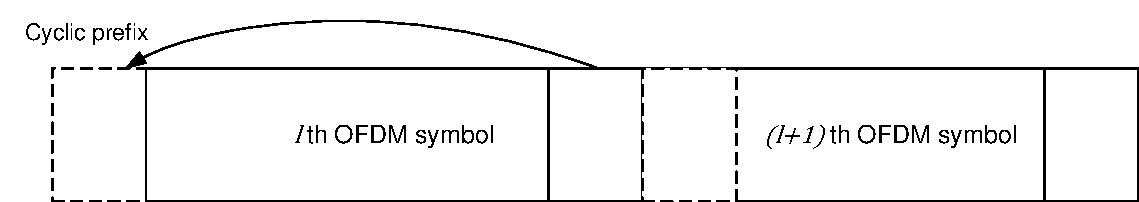
\includegraphics[width=0.8\textwidth]{images/Cyclic prefix.pdf}
        \caption{OFDM symbols with CP}
        \label{fig:CP}
    \end{figure}
    \item Reshape: Group the data for OFDM symbols using.
    \item AWGN Channel: \textit{Additive White Gaussian Noise} (AWGN) Channel can add noise to the signal. The noise is generated by a Gaussian distribution with a mean of zero and a standard deviation of 1. The noise power is controlled by the $Eb/No$ parameter.
\end{itemize}
As for the receiver, we only need to reverse the process of transmission and do some small modifications. In addition to the transceiver, I have added some blocks for testing.
\begin{itemize}
    \item Constellation Diagram: It can reveal modulation error rates, BER, phase noise, amplitude noise and other issues.
    \item Spectrum Analyzer: Observation of the signal spectrum using the FFT technique.
    \item Error Rate Calculation: This block can calculate the error rate and provide three groups of result which are the error rate, number of errors and the number of samples compared.
    \item Slider: This block can adjust the $Eb/No$ parameter in the AWGN Channel block very conveniently.
\end{itemize}
\section{BER Analysis}
\subsection{Constellation Diagram}
\begin{figure}[!h]
    \centering
    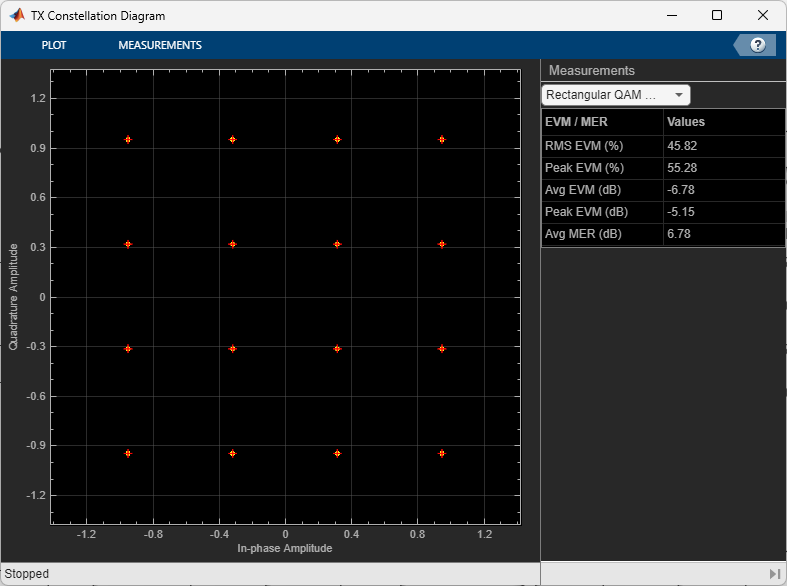
\includegraphics[width=0.5\textwidth]{images/TX Constellation Diagram.png}
    \caption{Constellation Diagram of Transmitter}
    \label{fig:TXConstellation}
\end{figure}
\begin{figure}[!h]
    \centering
    \subfigure[Constellation Diagram@25dB]{
        \begin{minipage}[b]{0.4\textwidth}
            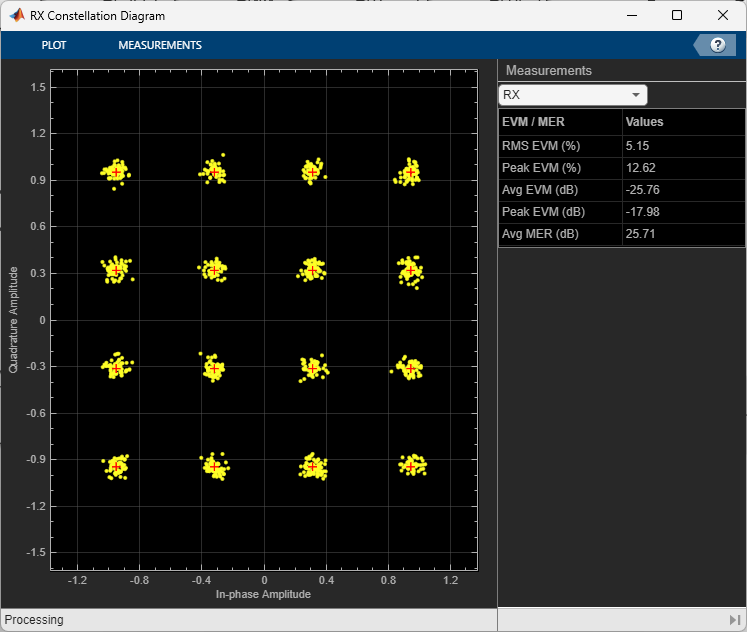
\includegraphics[width=1\textwidth]{images/RX Constellation Diagram25dB.png}
        \end{minipage}
    \label{fig:Receiver@25dB}
    }
    \subfigure[Constellation Diagram@0dB]{
        \begin{minipage}[b]{0.4\textwidth}
            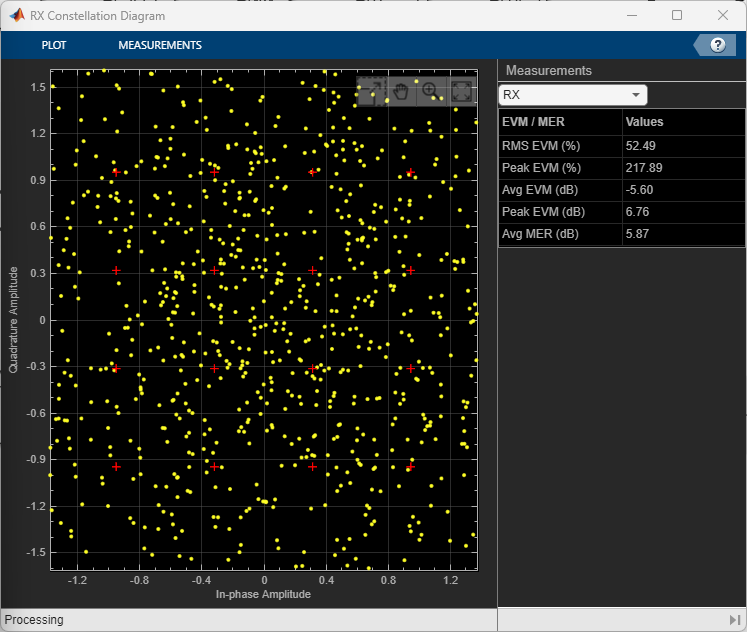
\includegraphics[width=1\textwidth]{images/RX Constellation Diagram0dB.png}
        \end{minipage}
    \label{fig:Receiver@0dB}
    }
    \caption{Constellation Diagram of Receiver}
    \label{fig:RXConstellation}
\end{figure}
The constellation diagrams are shown in Figure \ref{fig:TXConstellation} and Figure \ref{fig:RXConstellation}. In the figure we can clearly see that the \textit{Root Mean Square} (RMS) \textit{Error Vector Magnitude} (EVM) and Peak EVM are declined due to the reduced channel quality. The symbols have also become more dispersed.
\subsection{Power Spectrum}
\begin{figure}[!h]
    \centering
    \subfigure[Power Spectrum@25dB]{
    \begin{minipage}{1\textwidth}
        \centering
        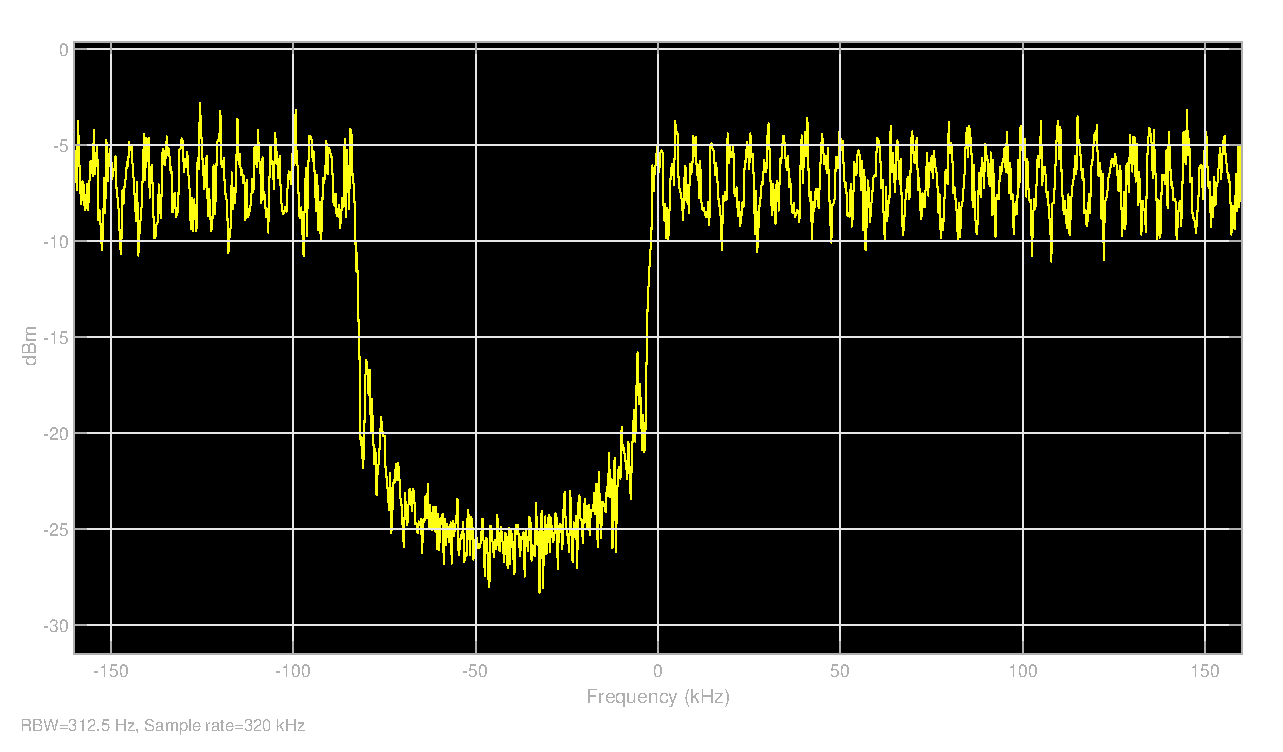
\includegraphics[scale=0.55]{images/spectrum25.eps}
    \end{minipage}
    }
    \subfigure[Power Spectrum@0dB]{
    \begin{minipage}{1\textwidth}
        \centering
        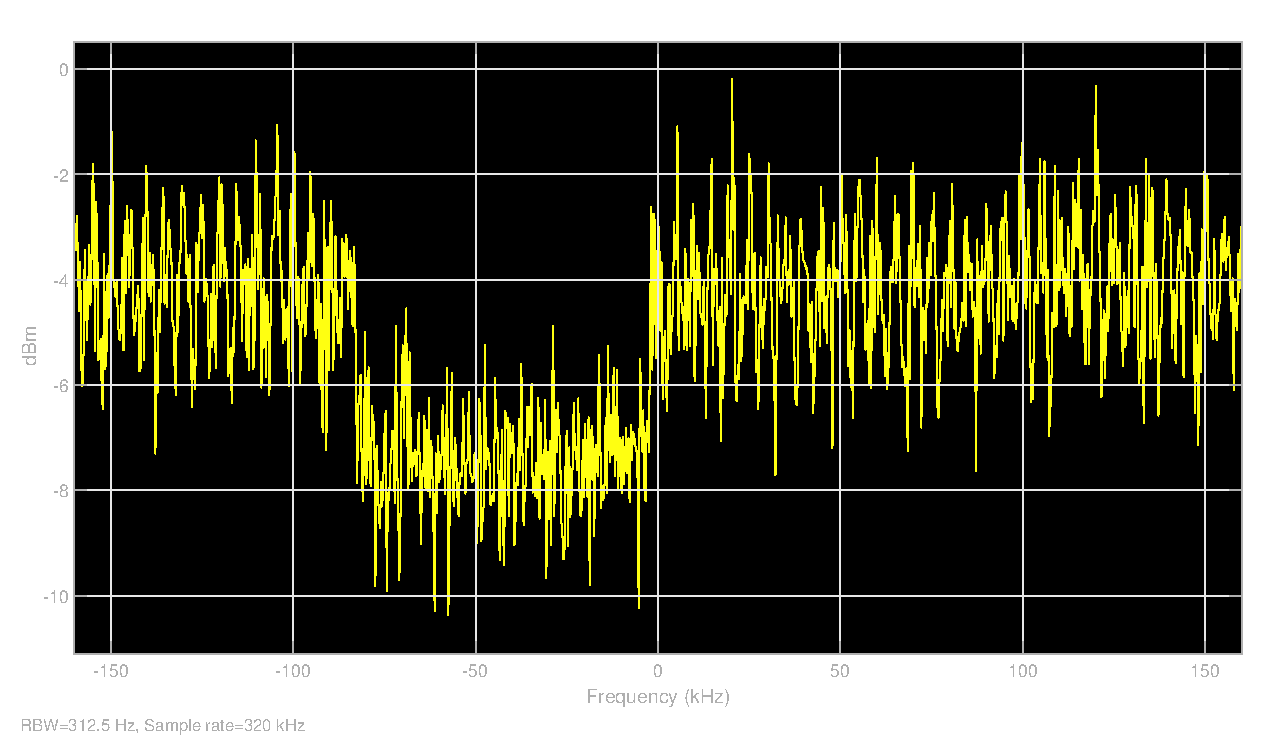
\includegraphics[scale=0.55]{images/spectrum0.eps}%
    \end{minipage}
    }
    \caption{Power Spectrum}
    \label{fig:Power Spectrum}
\end{figure}
By decreasing the SNR from $25dB$ to $0dB$, the power spectrum of the signal after AWGN channel is shown in Figure \ref{fig:Power Spectrum}. The power spectrum of the signal is reduced due to the reduced channel quality. The frequency spectrum of the signal also starts to become irregular.
\subsection{BER Curve}
Since I used the gain block in the OFDM model, the signal power of the AWGN input needs to be modified to 1 in the QAM only model so that the BER can be measured correctly.

In the model, I will use ``To Workspace'' block to save the result from the ``Error Rate Calculation'' block and plot the BER vs. $Eb/No$''.

In addition to setting $Eb/No$ to values of 0, 5, 10, 15, 20, 25 dB, I have additionally set $Eb/No$ to values in steps of 1 from 0 to 20 db. The BER corresponding to these values is recorded and plotted.

From the Figure \ref{fig:BER}, however, we can see that the BER of 16-QAM-based OFDM is worse than that of QAM-only after signal power normalization because the OFDM model has more blocks than the QAM-only model. The more blocks there are, the more errors there will be.In addition, the OFDM model has a cyclic prefix, which will cause the BER to increase. 

Comparing the channel between the AWGN channel and the Rayleigh fading channel, we can see that these two models will have a very low BER when they were transmitted under Rayleigh fading channel. The curves are almost indistinguishable and have no reference value. I believe it is caused by the wrong parameter setting of the Rayleigh fading block. I will try to fix it in the future.
\begin{figure}[!h]
    \centering
    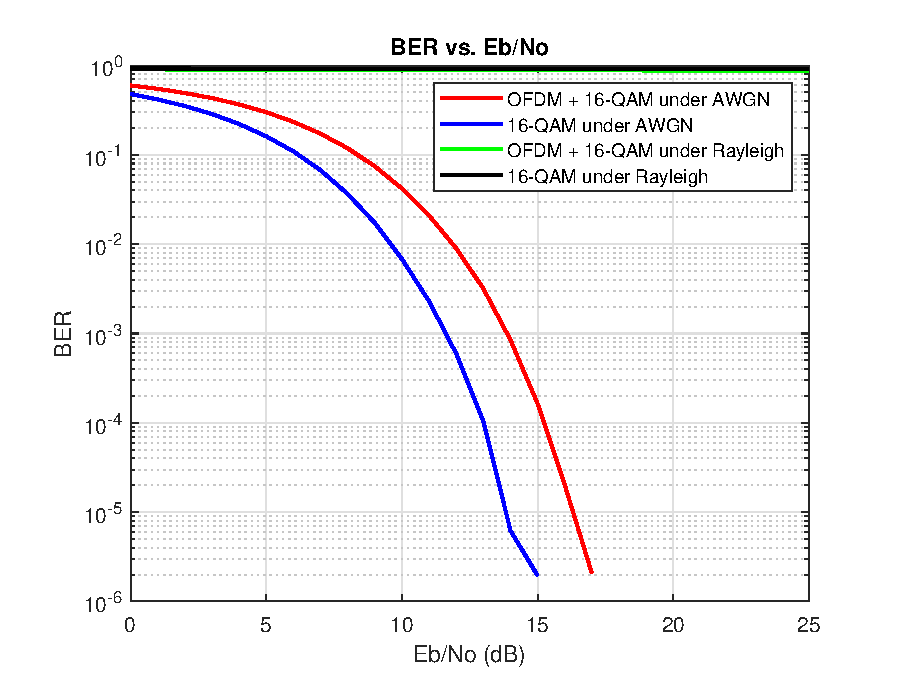
\includegraphics[width=0.8\textwidth]{images/BER.eps}
    \caption{BER vs. Eb/No}
    \label{fig:BER}
\end{figure}
\part{Conclusion}
In this report, I introduced the basic OFDM introduction and implementation, and also described the process of implementing 16-QAM based OFDM from Simulink$^\circledR$, and performed many tests including constellation diagram, power spectrum, and BER. The tests were carried out under different channel conditions. Theoretically, the BER should not be so low in the Rayleigh channel, probably due to the wrong parameter settings.
This project allowed us to build a good body of knowledge on OFDM and QAM and to exercise our Simulink$^\circledR$ simulation skills. We learned about the various factors that judge the quality of communication and the method of judging the quality.
In the future, the areas I need to improve are
\begin{itemize}
    \item Adjusting the parameters of Rayleigh fading channel
    \item Familiarize me with the correspondence between the module and the actual circuit
\end{itemize}
%%%%%%%%%%%%%%%%%%%%%%%%%%%%%%%%%%%%%%%%%%%%%%%
\pagebreak
\bibliographystyle{IEEEtran}
\bibliography{exportlist}
\addcontentsline{toc}{section}{References}

\end{document}